\documentclass[final,hyperref={pdfpagelabels=false},5pt]{beamer}
\usepackage{grffile}
\mode<presentation>{\usetheme{penn}}
\usepackage[english]{babel}
%\usepackage[latin1]{inputenc}
\usepackage{amsmath,amsthm, amssymb, latexsym}
%\usepackage{lmodern}
%\usepackage{times}\usefonttheme{professionalfonts}  % obsolete
%\usefonttheme[onlymath]{serif}
\boldmath
\usepackage[orientation=portrait,size=b1,scale=1.25,debug]{beamerposter}


\usepackage{rigidmath}
\usepackage{mathspec}
%\setmainfont{Times New Roman}
%\setsansfont[Ligatures=TeX, % recommended
   %UprightFont={* Light},
   %ItalicFont={* Light Italic},
   %BoldFont={*},
   %BoldItalicFont={* Italic}]{Open Sans}
%\setmainfont{Garamond Premier Pro}
%\setmathfont{Latin Modern Roman}
%\setmathfont[range=\mathit]{Latin Modern Roman}
%\setmathrm{Latin Modern Roman}
%\usepackage[default,osfigures]{opensans}
%\renewcommand\seriesdefault{l}
%\renewcommand\bfdefault{m}
%\setlength{\paperwidth}{30in}
%\setlength{\paperheight}{40in}
% change list indention level
% \setdefaultleftmargin{3em}{}{}{}{}{}


%\usepackage{snapshot} % will write a .dep file with all dependencies, allows for easy bundling

\usepackage{array,booktabs,tabularx}







\newcolumntype{Z}{>{\centering\arraybackslash}X} % centered tabularx columns
%\newcommand{\pphantom}{\textcolor{ta3aluminium}} % phantom introduces a vertical space in p formatted table columns??!!

\listfiles

%%%%%%%%%%%%%%%%%%%%%%%%%%%%%%%%%%%%%%%%%%%%%%%%%%%%%%%%%%%%%%%%%%%%%%%%%%%%%%%%%%%%%%
\graphicspath{{figures/}}
 
%\title{\fontspec{Garamond Premier Pro} { Modeling and Analysis of Non-unique Behaviors in Multiple Frictional Impacts }}
%\title{\fontspec{Garamond Premier Pro} {\noindent  \,MODELING AND ANALYSIS OF NON-UNIQUE\, \linebreak \mbox{\,BEHAVIORS} IN MULTIPLE FRICTIONAL IMPACTS\, \linebreak} }
%\title{{\noindent  \,MODELING AND ANALYSIS OF NON-UNIQUE\, \linebreak \mbox{\,BEHAVIORS} IN MULTIPLE FRICTIONAL IMPACTS\, \linebreak} }
\title{{\noindent  \,SAMPLE-EFFICIENT LEARNING OF \, \linebreak \,RIGID BODY DYNAMICS\, \linebreak} }
\author{Samuel Pfrommer, Mathew Halm, Michael Posa}
\institute[University of Pennsylvania]{DAIR Laboratory --- GRASP Laboratory --- University of Pennsylvania}
\date{Feb. 12th, 2018}

%%%%%%%%%%%%%%%%%%%%%%%%%%%%%%%%%%%%%%%%%%%%%%%%%%%%%%%%%%%%%%%%%%%%%%%%%%%%%%%%%%%%%%
\newlength{\columnheight}
\setlength{\columnheight}{31.5in}
%\useinnertheme{rounded}

%%%%%%%%%%%%%%%%%%%%%%%%%%%%%%%%%%%%%%%%%%%%%%%%%%%%%%%%%%%%%%%%%%%%%%%%%%%%%%%%%%%%%%
\begin{document}
\begin{frame}
  \vspace{-26ex}
    \begin{columns}
    % ---------------------------------------------------------%
    % Set up a column 
    \begin{column}{.49\textwidth}
      \begin{beamercolorbox}[center,wd=\textwidth]{postercolumn}
        \begin{minipage}[T]{.95\textwidth}  % tweaks the width, makes a new \textwidth
          \parbox[t][\columnheight]{\textwidth}{ % must be some better way to set the the height, width and textwidth simultaneously
            % Since all columns are the same length, it is all nice and tidy.  You have to get the height empirically
            % ---------------------------------------------------------%
            % fill each column with content  
            \begin{block}{Motivation}
              \color{penndkbl}
                    \begin{itemize}
                        \item Current robots are stuck in repetitive, predictable environments
                        \item Want to enable dynamic interaction with objects
                        \item Frictional contact is fundamental to robot manipulation, but difficult to model
                            \begin{itemize}
                                \item Sudden changes in dynamics when making/breaking contact 
                                \item Inconsistencies with Coulomb friction (Painlev\'{e} paradox)
                                \item Many simultaneous contacts
                                \item Stick/slip transitions
                            \end{itemize}
                    \end{itemize}
              \end{block}
                      
            \begin{block}{Prior Work}
                \begin{columns}[t]
                    \begin{column}{0.3\textwidth}
                        \textbf{Learned}
                        \begin{itemize}
                            \item Often in context of policy learning
                            \item Slow and data innefficient
                            \item Doesn't use existing knowledge of contact dynamics
                        \end{itemize}
                    \end{column}

                    \begin{column}{0.3\textwidth}
                        \textbf{Hybrid}
                        \begin{itemize}
                            \item Best of both worlds
                        \end{itemize}
                        \begin{center}
                            \textit{Approaches:}
                        \end{center}
                        \begin{itemize}
                            \item Sim-to-real
                            \item Residual physics
                            \item \textbf{Differentiation through contact problem}
                        \end{itemize}
                    \end{column}

                    \begin{column}{0.3\textwidth}
                        \textbf{Analytical}
                        \begin{itemize}
                            \item Only an approximation
                            \item Doesn't fully capture real-world phenomena
                        \end{itemize}
                    \end{column}
                \end{columns}
            \end{block}
            

            \begin{block}{Method}
            	\begin{figure}
	              	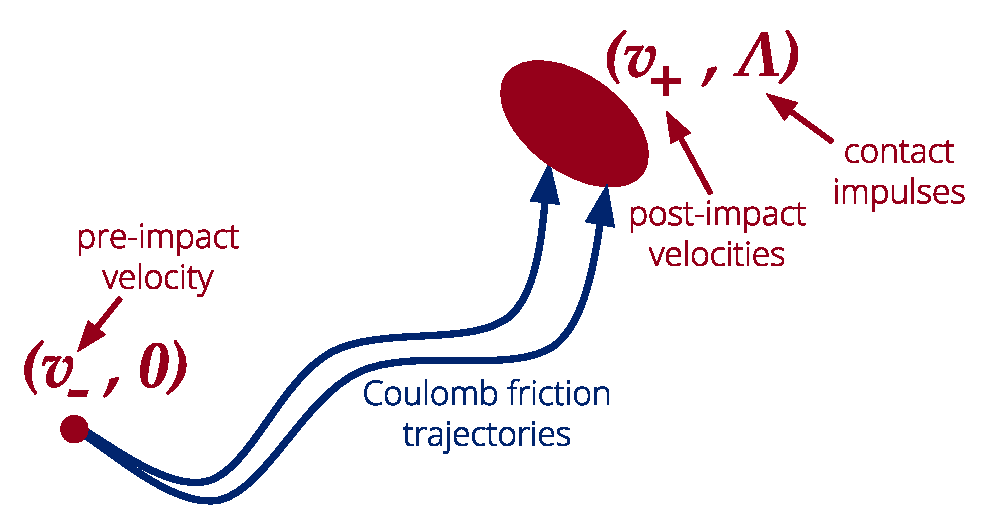
\includegraphics[width=0.7\textwidth]{VelocityConnection}
	              \end{figure}
              \begin{itemize}
              \item Finds change in velocity and impulses via Newton's second law:
	                  $$\Mass (\Velocity_+ - \Velocity_-) = \J^T \Impulse$$
	              \item Extension of Routh's 1891 model to multiple contacts \cite{Routh91}
	              
	              \item $\Velocity_+$ and $\Impulse$ determined \textit{incrementally}:
	              
	              \begin{enumerate}
	              	\item Increase normal impulses with slopes $\NormalForce[i]$ such that
	              		$$\sum_i \NormalForce[i] = 1$$
	              	\item Increment each friction impulse via Coulomb friction:
	             		$$\TwoNorm{\FrictionForce[i]} \leq \FrictionCoeff[i]\Norm{\NormalForce[i]},\qquad \FrictionForce[i] \in \arg \min_{\FrictionForce[i]} \FrictionForce[i]^T\Velocity_i$$
	              	\item Terminate when $\Velocity = \Velocity_- + \Mass^{-1}\J^T \Lambda$ no longer penetrates
	              \end{enumerate}
	              \item
	              Formulation as a \textit{differential inclusion}
	              $$\frac{\mathrm{d}}{\mathrm{d}s} \Velocity(s) \in D(\Velocity(s))$$
              \end{itemize}
            \end{block}
            \footnotesize{\color{pennbl}
				\bibliography{library}
				\bibliographystyle{plain}}
           \begin{columns}[c]
				\begin{column}{.25\textwidth}
				
				\begin{figure}
				
					
\includegraphics[width=\textwidth]{NSFLogo}
				\end{figure}
				\end{column}
				\begin{column}{.64\textwidth}
				\centering
				\begin{figure}
				\centering
					
\includegraphics[width=\textwidth]{grasp_logo1_blue}
				\end{figure}

				\end{column}
				\end{columns}
				

    
          }
        \end{minipage}
        
      \end{beamercolorbox}
      
    \end{column}
    %\textcolor{penndkbl}{\vrule}

\hfill
    % ---------------------------------------------------------%
    % end the column

    % ---------------------------------------------------------%
    % Set up a column 
    \begin{column}{.49\textwidth}
      \begin{beamercolorbox}[center,wd=\textwidth]{postercolumn}
        \begin{minipage}[T]{.95\textwidth} % tweaks the width, makes a new \textwidth
          \parbox[t][\columnheight]{\textwidth}{ % must be some better way to set the the height, width and textwidth simultaneously
            % Since all columns are the same length, it is all nice and tidy.  You have to get the height empirically
            % ---------------------------------------------------------%
            % fill each column with content
             \begin{block}{Theoretical Results}
             \begin{center}
             	\textbf{Model is proven to be well behaved:}
             \end{center}
              \begin{itemize}
              \item Dissipation of kinetic energy $\KineticEnergy(s)$, \textbf{but} no guaranteed rate $\TotalDiff{}{s}\KineticEnergy < - \varepsilon K$
               $$\KineticEnergy (s + k) \leq \KineticEnergy (s),\, \forall k > 0$$
              \item Homogeneity of impact map
              	$$\Parentheses{\Velocity_- \to \Velocity_+} \implies \Parentheses{k\Velocity_- \to k\Velocity_+,\, \forall k \geq 0}$$
              \item \textbf{Existence of solutions} to every initial value problem
              \end{itemize}
              \vspace{1ex}
              \begin{center}
               \textbf{\color{pennrd} Antagonistic scenarios may prevent finding valid post-impact state:}
               \end{center}
              \begin{figure}
              	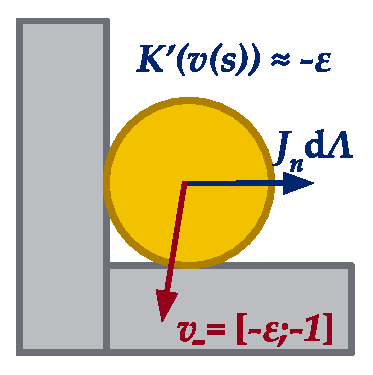
\includegraphics[width=0.3\textwidth]{Corner}
              	\hspace{0.125\textwidth}
              	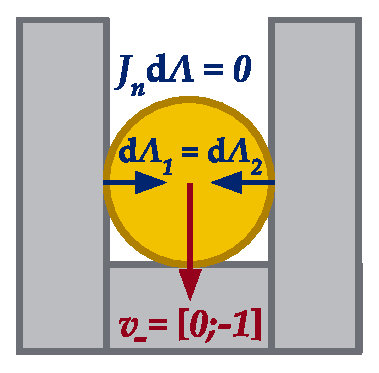
\includegraphics[width=0.3\textwidth]{Bucket}
              \end{figure}
              \begin{tcolorbox}[colback=pennyw,
colframe=penndyw,boxrule=5pt,coltext=pennbl,outer arc=5pt,arc=0pt]
              \textbf{Theorem.} For non-jammed systems, impact terminates linearly in $\Norm{\Velocity(0)}$.	
              \end{tcolorbox}     
            \end{block}
            
             \begin{block}{Application: Rimless Wheel}
             \centering
             \begin{columns}[c]
				\begin{column}{.47\hsize}
				\justify
				Impact model not only gives each of the three first-principles results, but also returns every reasonable \mbox{intermediate} result.
				\end{column}
				\begin{column}{.47\hsize}
				\centering
				\vspace{0ex}
				\begin{figure}
				\centering
              	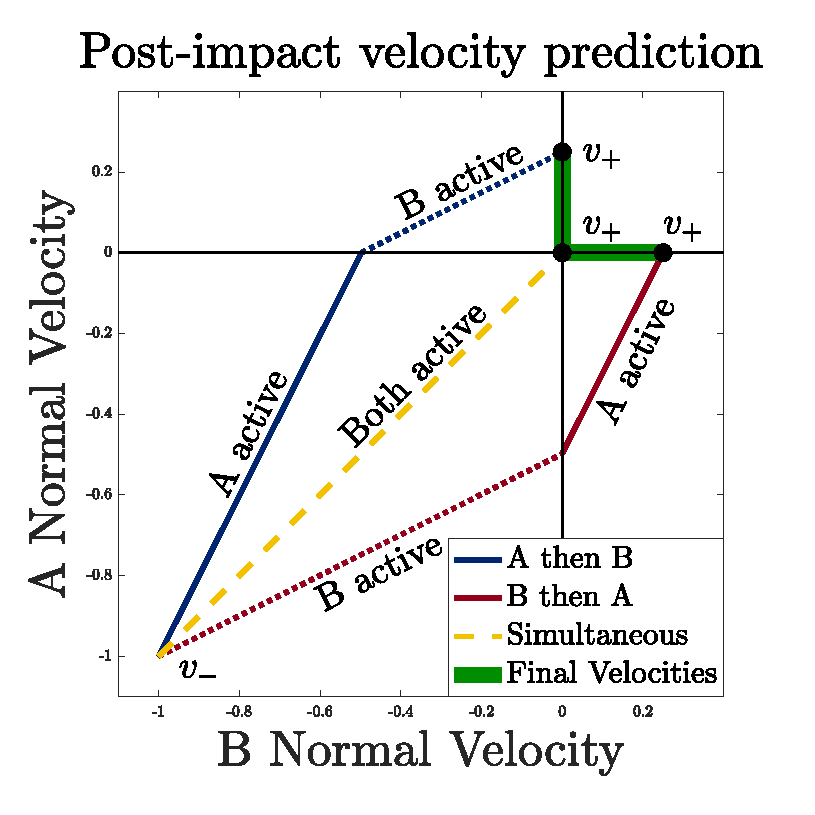
\includegraphics[width=0.8\textwidth]{rimless_example_2_4}
              	\end{figure} 
				\end{column}
				\end{columns}
             \centering
             \end{block}
             
             \begin{block}{Application: Manipulation}
             \centering
             \begin{columns}[c]
             
				\begin{column}{.47\hsize}
				\justify
				Non-uniqueness emerges even without simultaneous impact. A block slid into a wall (right) will have sensitive behaviors due to propagation of shockwaves through the body.
				\end{column}
				\begin{column}{.47\hsize}
				\centering
				\vspace{0ex}
				\begin{figure}
				\centering
              	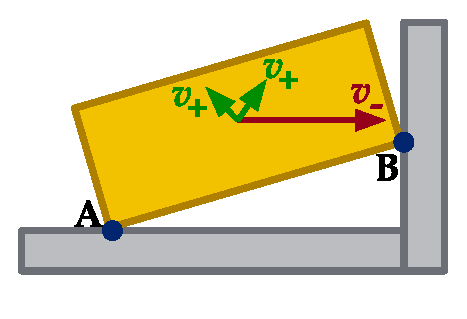
\includegraphics[width=0.9\textwidth]{PushingFinal}
              	\end{figure} 
				\end{column}
				\end{columns}
				\begin{figure}
					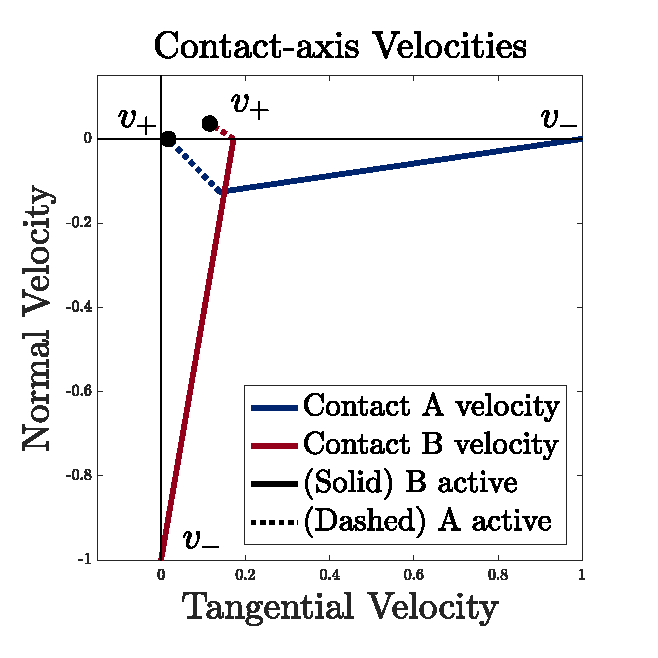
\includegraphics[width=0.4\textwidth]{pushing_example_1}
					\hspace{0.06\textwidth}
					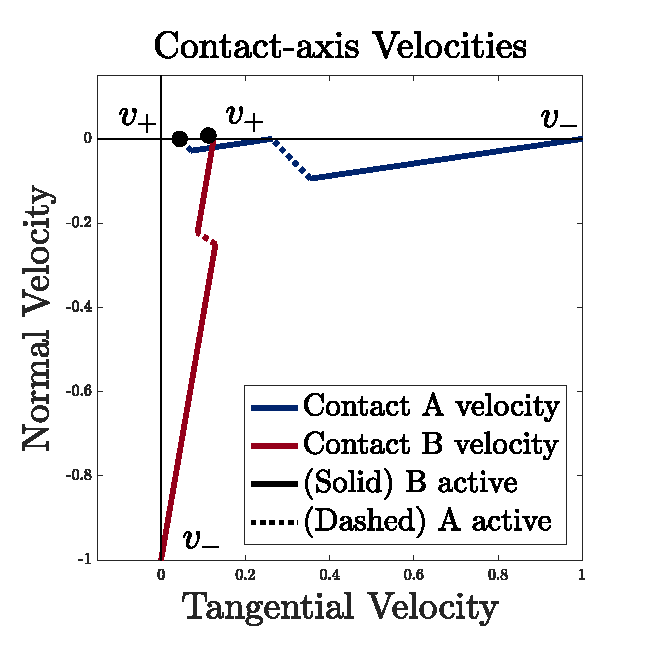
\includegraphics[width=0.4\textwidth]{pushing_example_2}
				\end{figure}
            \end{block}
            
             \begin{block}{Summary}
             \textbf{Contributions}
              \begin{itemize}
              \item Derivation of a simultaneous inelastic impact model
              \item Proven characterization of model properties
              \item Guarantees for existence of solutions and impact termination
              \end{itemize}
              \vspace{1ex}
               \textbf{Ongoing Work}             
              \begin{itemize}
              \item Modeling of elastic impacts
              \item Embedding impact model into full dynamics
              \item Time-stepping simulation through impact
              \item Algorithms for approximating post-impact set
              \end{itemize}
            \end{block}
            
          }
          % ---------------------------------------------------------%
          % end the column
        \end{minipage}
      \end{beamercolorbox}
    \end{column}
    % ---------------------------------------------------------%
    % end the column
  \end{columns}
  
%  \begin{center} 
%  \begin{minipage}{.85 \textwidth}
%  \begin{block}{References}
%  {
%  \scriptsize
%\bibliography{library}
%\bibliographystyle{plain}
%}
%  \end{block}   
%    \end{minipage}   
%   \end{center}
   
\end{frame}
\end{document}
